\documentclass{article}

\makeatletter

\usepackage{calc}
\usepackage{xcolor}

\usepackage{fontspec}
\defaultfontfeatures{Ligatures={TeX}}

\setmainfont[
  ItalicFont = Crimson Italic,
  BoldFont = Crimson Semibold,
  BoldItalicFont = Crimson SemiboldItalic,
  Numbers = Lining,
]{Crimson Roman}

\usepackage{geometry}
\geometry{
  paperwidth=18cm,
  paperheight=5cm,
  hmargin=0pt,
  vmargin=0pt,
  noheadfoot,
  centering,
}

\definecolor{base03}{HTML}{002B36}
\definecolor{base02}{HTML}{073642}
\definecolor{base01}{HTML}{586E75}
\definecolor{base00}{HTML}{657B83}
\definecolor{base0}{HTML}{839496}
\definecolor{base1}{HTML}{93A1A1}
\definecolor{base2}{HTML}{EEE8D5}
\definecolor{base3}{HTML}{FDF6E3}
\definecolor{yellow}{HTML}{B58900}
\definecolor{orange}{HTML}{CB4B16}
\definecolor{red}{HTML}{DC322F}
\definecolor{magenta}{HTML}{D33682}
\definecolor{violet}{HTML}{6C71C4}
\definecolor{blue}{HTML}{268BD2}
\definecolor{cyan}{HTML}{2AA198}
\definecolor{green}{HTML}{859900}

\colorlet{background}{base3}
\colorlet{primary-content}{base00}
\colorlet{bg-highlight}{base2}
\colorlet{secondary-content}{base1}
%\colorlet{list-content}{base0}
\colorlet{list-content}{primary-content}
\colorlet{list-bullets}{orange}
\colorlet{lvl1-color}{primary-content}
\colorlet{lvl2-color}{primary-content}
\colorlet{lvl3-color}{yellow}
\colorlet{lvl4-color}{green}

\usepackage{tikz}
\usetikzlibrary{calendar}
\usetikzlibrary{positioning}
\usetikzlibrary{shapes.geometric}

\usepackage{wasysym}

\newcommand*\moonformat[1]{{\color{primary-content} #1}}

\newcommand\GaNewmoon{\moonformat{\CIRCLE}}
\newcommand\GaWaxingmoon{\moonformat{\LEFTcircle}}
\newcommand\GaFullmoon{\moonformat{\Circle}}
\newcommand\GaWaningmoon{\moonformat{\RIGHTcircle}}

\newcommand*\datenumsize{\@setfontsize\datenumsize{10}{12}}
\newcommand*\monthlabelsize{\@setfontsize\monthlabelsize{10}{12}}
\newcommand*\datedaysize{\@setfontsize\datedaysize{8}{11}}

\newcommand*\datedayFormat[1]{\datedaysize #1}

\tikzstyle{planner}=[
  month list,
  day xshift=4.5mm,
  month yshift=15mm,
  every month/.append style={anchor=base, inner xsep=0pt},
  month text={\monthlabelsize\color{primary-content}\%y0 \%m.},
  day text={\datenumsize\%d-},
  every day/.append style={anchor=base, inner xsep=0pt},
  month label left,
  execute at begin day scope={
    \ifdate{Sunday}{\color{black!60}}{}
  }
]

\newcommand{\moondays}{%
if (equals=2016-01-02) [day text=\GaWaningmoon]%
if (equals=2016-01-08) [day text=\GaNewmoon]%
if (equals=2016-01-16) [day text=\GaWaxingmoon]%
if (equals=2016-01-23) [day text=\GaFullmoon]%
if (equals=2016-01-31) [day text=\GaWaningmoon]%
if (equals=2016-02-07) [day text=\GaNewmoon]%
if (equals=2016-02-15) [day text=\GaWaxingmoon]%
if (equals=2016-02-22) [day text=\GaFullmoon]%
if (equals=2016-03-01) [day text=\GaWaningmoon]%
if (equals=2016-03-07) [day text=\GaNewmoon]%
if (equals=2016-03-15) [day text=\GaWaxingmoon]%
if (equals=2016-03-22) [day text=\GaFullmoon]%
if (equals=2016-03-30) [day text=\GaWaningmoon]%
if (equals=2016-04-06) [day text=\GaNewmoon]%
if (equals=2016-04-14) [day text=\GaWaxingmoon]%
if (equals=2016-04-21) [day text=\GaFullmoon]%
if (equals=2016-04-29) [day text=\GaWaningmoon]%
if (equals=2016-05-05) [day text=\GaNewmoon]%
if (equals=2016-05-13) [day text=\GaWaxingmoon]%
if (equals=2016-05-20) [day text=\GaFullmoon]%
if (equals=2016-05-28) [day text=\GaWaningmoon]%
if (equals=2016-06-04) [day text=\GaNewmoon]%
if (equals=2016-06-12) [day text=\GaWaxingmoon]%
if (equals=2016-06-19) [day text=\GaFullmoon]%
if (equals=2016-06-27) [day text=\GaWaningmoon]%
if (equals=2016-07-04) [day text=\GaNewmoon]%
if (equals=2016-07-12) [day text=\GaWaxingmoon]%
if (equals=2016-07-19) [day text=\GaFullmoon]%
if (equals=2016-07-27) [day text=\GaWaningmoon]%
if (equals=2016-08-03) [day text=\GaNewmoon]%
if (equals=2016-08-11) [day text=\GaWaxingmoon]%
if (equals=2016-08-18) [day text=\GaFullmoon]%
if (equals=2016-08-26) [day text=\GaWaningmoon]%
if (equals=2016-09-01) [day text=\GaNewmoon]%
if (equals=2016-09-09) [day text=\GaWaxingmoon]%
if (equals=2016-09-16) [day text=\GaFullmoon]%
if (equals=2016-09-24) [day text=\GaWaningmoon]%
if (equals=2016-10-01) [day text=\GaNewmoon]%
if (equals=2016-10-09) [day text=\GaWaxingmoon]%
if (equals=2016-10-16) [day text=\GaFullmoon]%
if (equals=2016-10-24) [day text=\GaWaningmoon]%
if (equals=2016-10-30) [day text=\GaNewmoon]%
if (equals=2016-11-07) [day text=\GaWaxingmoon]%
if (equals=2016-11-14) [day text=\GaFullmoon]%
if (equals=2016-11-22) [day text=\GaWaningmoon]%
if (equals=2016-11-29) [day text=\GaNewmoon]%
if (equals=2016-12-07) [day text=\GaWaxingmoon]%
if (equals=2016-12-14) [day text=\GaFullmoon]%
if (equals=2016-12-22) [day text=\GaWaningmoon]%
if (equals=2016-12-28) [day text=\GaNewmoon]%
}

\setlength{\parindent}{0pt}

\usepackage{graphicx}

\makeatother

\begin{document}

\thispagestyle{empty}\mbox{}
\raggedright

\resizebox{\linewidth}{!}{%
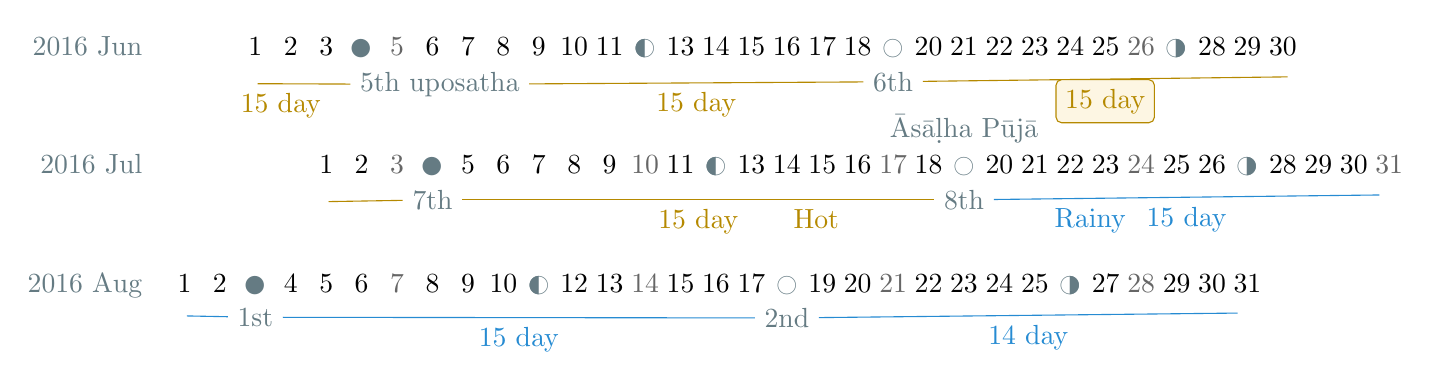
\begin{tikzpicture}[
    hot-interval-line/.style={ draw=yellow },
    hot-label/.style={ color=yellow, midway, below },
    hot-uposatha/.style={ color=primary-content },
    rainy-interval-line/.style={ draw=blue },
    rainy-label/.style={ color=blue, midway, below },
    rainy-uposatha/.style={ color=primary-content },
  ]

\calendar (cal) [dates=2016-06-01 to 2016-08-31, planner] \moondays;

\node (jun-a) [below=3pt of cal-2016-06-01.south west] {};
\node (u5) [hot-uposatha, below=-2pt of cal-2016-06-04.south west, anchor=north west] {5th uposatha};
\node (u6) [hot-uposatha, below=-2pt of cal-2016-06-19.south] {6th};
\node (jun-b) [below=0.5pt of cal-2016-06-30.south east] {};
\node (u7) [hot-uposatha, below=-2pt of cal-2016-07-04.south] {7th};
\node (jul-a) [below=3pt of cal-2016-07-01.south west] {};
\node (u8) [hot-uposatha, below=-2pt of cal-2016-07-19.south] {8th};

\node (asalha) [primary-content, above=-2pt of cal-2016-07-19.north] {Āsāḷha Pūjā};

node [blue, below=-2pt of cal-2016-07-19.south east, anchor=north west] {Rainy};

\draw [hot-interval-line] (jun-a) -- (u5) node[hot-label, near start] {15 day};
\draw [hot-interval-line] (u5) -- (u6) node[hot-label] {15 day};
\draw [hot-interval-line] (u6) -- (jun-b) node[hot-label, fill=background, rounded corners=2pt, draw=yellow] {15 day};
\draw [hot-interval-line] (jul-a) -- (u7);
\draw [hot-interval-line] (u7) -- (u8)
  node[hot-label] {15 day}
  node [hot-label, near end] {Hot};

\node (jul-b) [below=0.5pt of cal-2016-07-31.south] {};
\node (aug-a) [below=1.5pt of cal-2016-08-01.south west] {};
\node (ru1) [rainy-uposatha, below=-2pt of cal-2016-08-03.south] {1st};
\node (ru2) [rainy-uposatha, below=-2pt of cal-2016-08-18.south] {2nd};
\node (aug-b) [below=0.5pt of cal-2016-08-31.south] {};

\draw [rainy-interval-line] (u8) -- (jul-b)
  node[rainy-label] {15 day}
  node[rainy-label, near start] {Rainy};
\draw [rainy-interval-line] (aug-a) -- (ru1);
\draw [rainy-interval-line] (ru1) -- (ru2) node[rainy-label] {15 day};
\draw [rainy-interval-line] (ru2) -- (aug-b) node[rainy-label] {14 day};

\end{tikzpicture}%
}

\end{document}
